\subsection{Statistically comparing the performance of the two best performing models}

The estimated generalization errors of the three different classification models, are outlined in table \ref{classification-performance}. The two models with the lowest estimated generalization errors are \textit{K-nearest neighbors} and \textit{Decision tree} respectively. These models will be used for the comparison, even though it is not known which models are best before the statistical analysis itself. The evaluation will be using the evaluation procedure for comparing two classifiers as outlined in section 9.3.3 in the course notes \cite{coursenotes}. Much like in section \ref{sec:linreg_evaluation} we will use t-test with the hypothesis of the two models not being significantly different, and recheck it by inspecting the credibility intervals for the difference in prediction errors.

From the t-test based on the generalization errors in percentage for the two models we get a p-value of 0.711 meaning we cannot reject the hypothesis, and therefore we cannot say if the two models are significantly different. Calculating the credibility interval we get $[-5.15, 1.10]$, which clearly contains 0, confirming our result from the t-test. The performance of the two models are not distinguishable.

Comparing the two models to a dummy model which always predicts the glass type as the most populated class, we get the p-values with order of magnitude of $10^{-8}$, meaning that the hypothesis can be rejected, and the models are therefore significantly different from the dummy model. Looking at the credibility intervals we get $[-40.52, -34.80]$ and $[-38.77, -32.49]$ clearly showing that the intervals do not contain 0, also, like in section \ref{sec:linreg_evaluation}, we see that the intervals only span negative numbers, showing that the prediction errors of the two models are significantly lower than those of the dummy model.

Comparisons of the cross-validation errors in percentage between the two classifier models and the largest class predicting model are seen in figure \ref{fig:cv_clas}.

\begin{figure}[H]
    \centering
    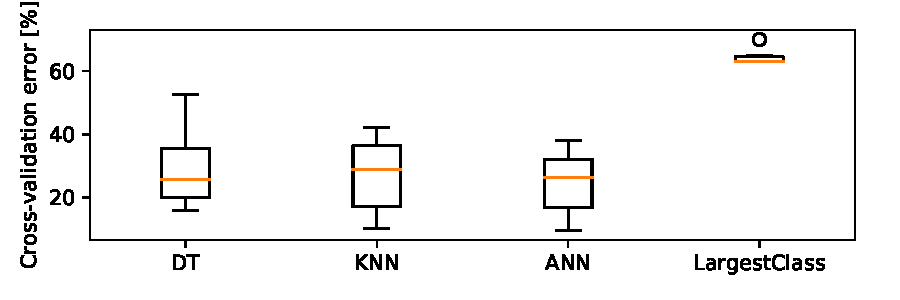
\includegraphics[width=0.7\textwidth]{fig/ClassifierEvaluation.pdf}
    \caption{Comparisons of the prediction errors obtained by cross validation between the different models: Decision tree, K-nearest neighbors, Artificial neural network and a model which always predicts the largest class.}
    \label{fig:cv_clas}
\end{figure}

Figure \ref{fig:cv_clas}, and the credibility intervals calculated above clearly shows that the two classification models outperforms the dummy model. Though it is also clear that since both models have an average generalization error at around 25\%-30\% that it is not an easy task to predict the glass type from the glass composition and refractive index alone. 